%%%%%%%%%%%%%%%%%%%%%%%%%%%%%%%%%%%%%%%%%%%%%%%%%%%%%%
%%%%%%%%%%%%%%%%%%%%%%%%%%%%%%%%%%%%%%%%%%%%%%%%%%%%%%
%%%%%%%%%%%%%%%%%%%%%%%%%%%%%%%%%%%%%%%%%%%%%%%%%%%%%%
%% \subsection{Shift $<\mu>$ by 1}

\begin{figure}[bt]
\centering
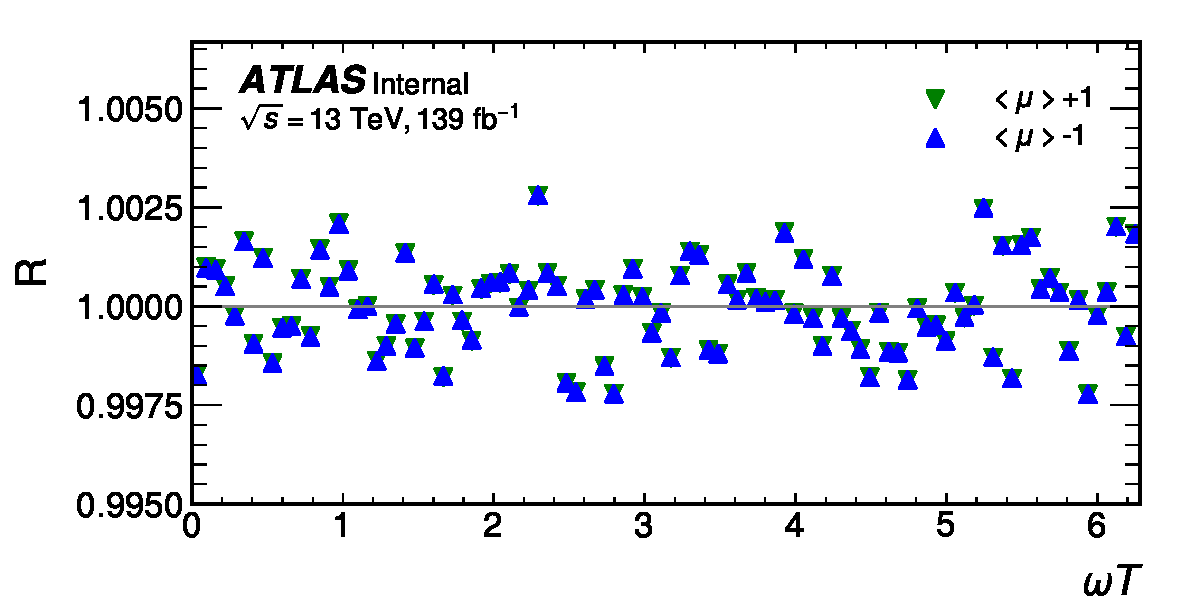
\includegraphics[width=0.95\textwidth]{figs/FMC_sys/compare_input_toy_datasets_mu_shifts} \\
\caption{ Comparison of the toy dataset with average pileup $<\mu>$ increased and decreased by 1. The toy dataset corresponds to four years of Run 2 luminosity is used. The X-axis is the sidereal phase, $\omega T$.
}
\label{fig:FMC_variation}
\end{figure}


\begin{figure}[bt]
\centering
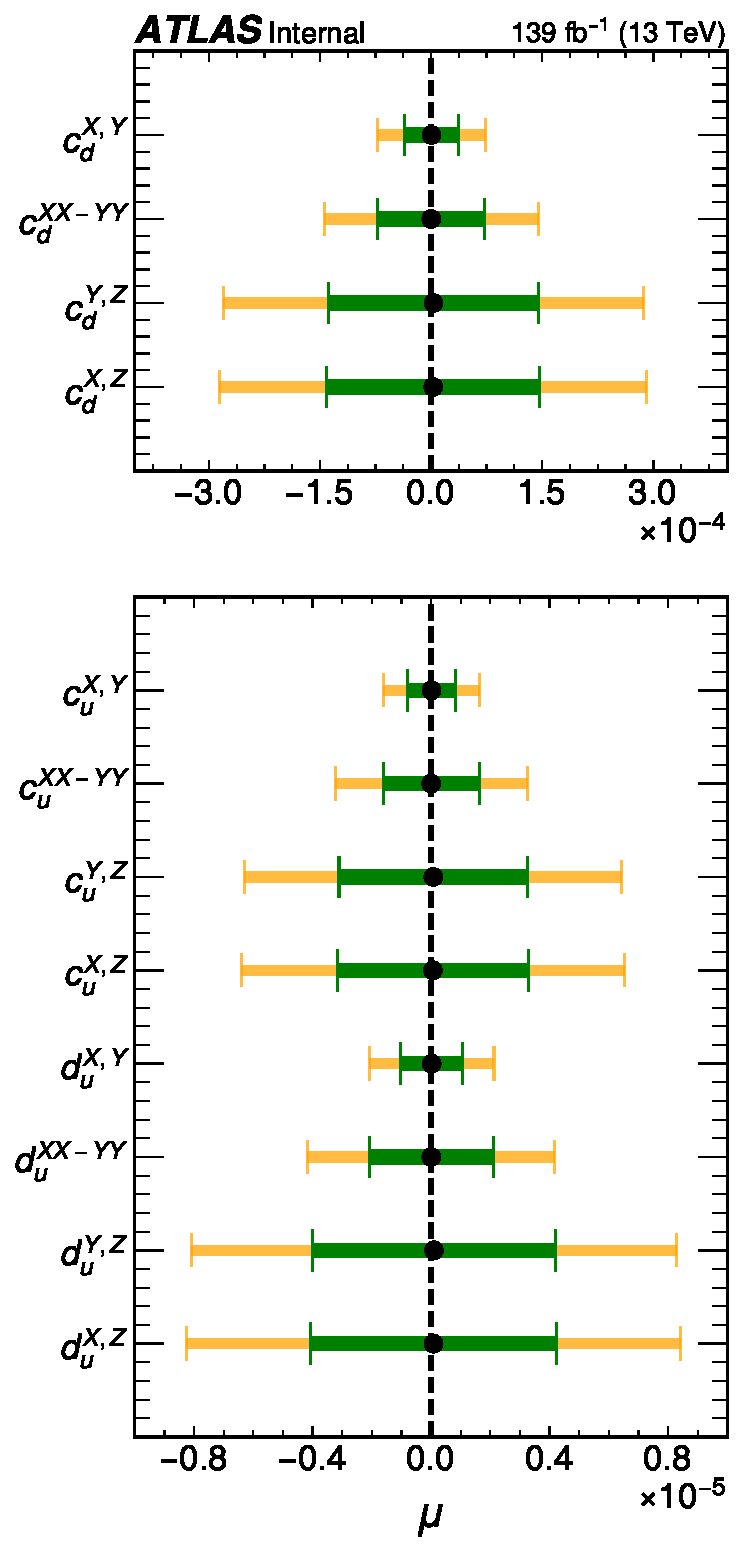
\includegraphics[width=0.4\textwidth]{figs/FMC_sys/SigFit_summary_AllSamples_muShift_p1} 
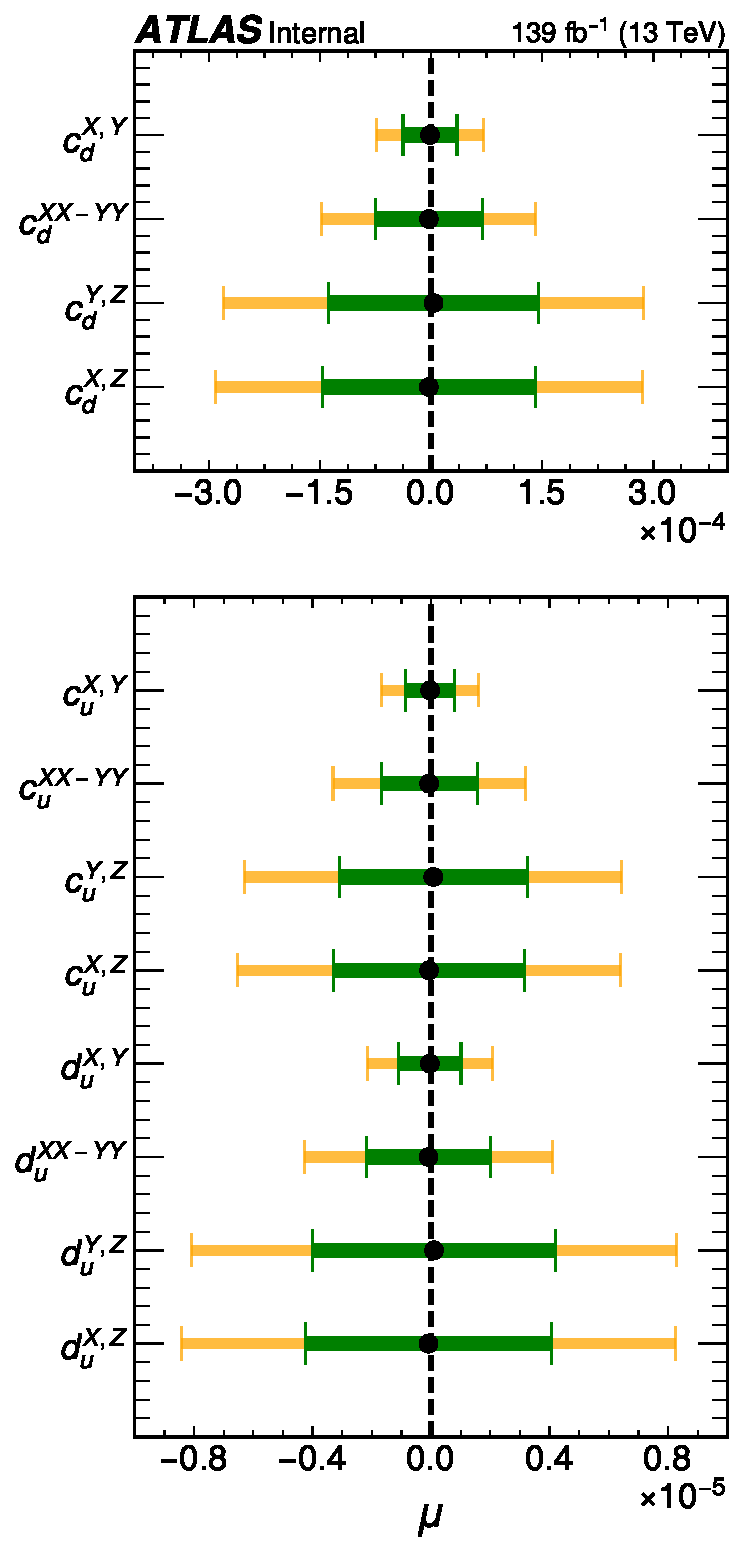
\includegraphics[width=0.4\textwidth]{figs/FMC_sys/SigFit_summary_AllSamples_muShift_m1} 
\caption{ Comparison of the fit results with average pileup $<\mu>$ increased and decreased by 1; left (+1) and right (-1). Results are obtained from 1000 toy datasets corresponding to four years of Run 2 luminosity. The X-axis is the sidereal phase, $\omega T$.
}
\label{fig:FMC_variation_summary}
\end{figure}
